% Taken from https://tex.stackexchange.com/questions/436259/timeline-in-latex

\documentclass[border=2mm]{standalone}

\usepackage{tikz}
\usetikzlibrary{decorations.pathreplacing}

\definecolor{myLightGray}{RGB}{191,191,191}
\definecolor{myGray}{RGB}{160,160,160}
\definecolor{myDarkGray}{RGB}{144,144,144}
\definecolor{myDarkRed}{RGB}{167,114,115}
\definecolor{myRed}{RGB}{255,58,70}
\definecolor{myGreen}{RGB}{0,255,71}

\begin{document}

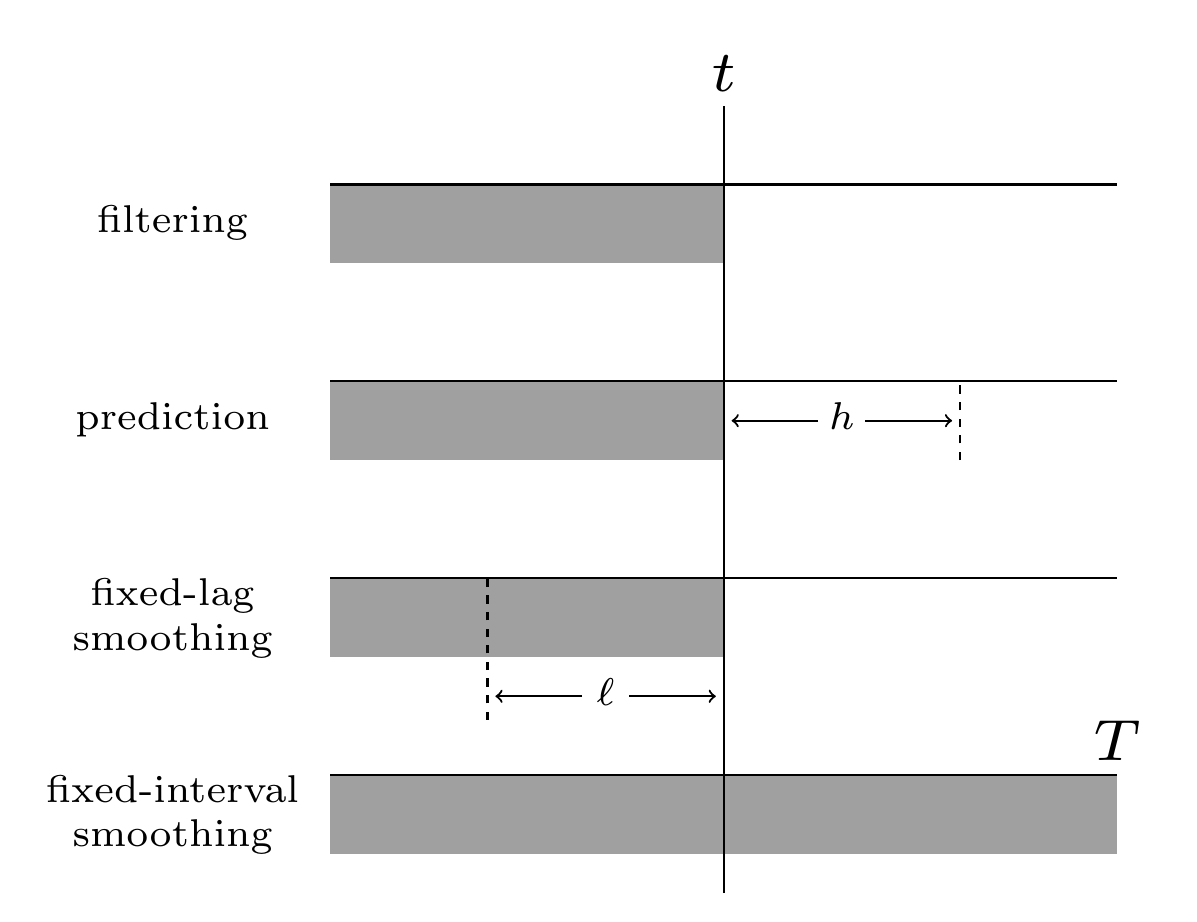
\begin{tikzpicture}[%
    every node/.style={
        font=\scriptsize,
        % Better alignment, see https://tex.stackexchange.com/questions/315075
        text height=1ex,
        text depth=.25ex,
    },
]
% place rectangles
\fill[myGray] (0,0.5) rectangle (10,1.5);
\fill[myGray] (0,3) rectangle (5,4);
\fill[myGray] (0,5.5) rectangle (5,6.5);
\fill[myGray] (0,8) rectangle (5,9);

% place axis labels
\node[anchor=south,scale=3] at (5,9.7) {$t$};
\node[anchor=south,scale=3] at (10,1.2) {$T$};
\node[align=center,scale=2] at (-2,0.7) {fixed-interval\\smoothing};
\node[align=center,scale=2] at (-2,3.2) {fixed-lag\\smoothing};
\node[scale=2] at (-2,6) {prediction};
\node[scale=2] at (-2,8.5) {filtering};

% place fixed-lag smoothing lines
\node[scale=2] at (3.5,2.5) {$\ell$};
\draw [thick, dashed] (2,2.2) -- (2,4);
\draw [thick, ->] (3.2,2.5) -- (2.1,2.5);
\draw [thick, ->] (3.8,2.5) -- (4.9,2.5);

% place prediction lines
\node[scale=2] at (6.5,6) {$h$};
\draw [thick, dashed] (8,5.5) -- (8,6.5);
\draw [thick, ->] (6.2,6) -- (5.1,6);
\draw [thick, ->] (6.8,6) -- (7.9,6);

% draw vertical line
\draw [thick] (5,0) -- (5,10);

% draw horizontal lines
\foreach \x in {1.5,4,6.5,9} {
    \draw [thick] (0,\x) -- (10, \x);
}

\end{tikzpicture}
\end{document}
